

\begin{figure}[h]

\centering






\tikzset{every picture/.style={line width=0.75pt}} %set default line width to 0.75pt        

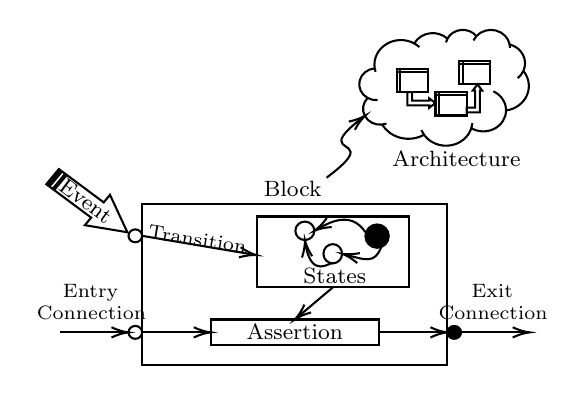
\begin{tikzpicture}[x=0.75pt,y=0.75pt,yscale=-0.75,xscale=0.75]
%uncomment if require: \path (0,300); %set diagram left start at 0, and has height of 300

%Shape: Rectangle [id:dp20254905050808336] 
\draw   (396.53,136.63) -- (592.69,136.63) -- (592.69,240) -- (396.53,240) -- cycle ;
%Shape: Rectangle [id:dp36813450527144953] 
\draw   (440.66,211.06) -- (548.55,211.06) -- (548.55,227.6) -- (440.66,227.6) -- cycle ;
%Shape: Rectangle [id:dp47798452515982937] 
\draw   (470.09,144.9) -- (568.17,144.9) -- (568.17,190.38) -- (470.09,190.38) -- cycle ;
%Straight Lines [id:da19778555219971472] 
\draw    (396.53,219.33) -- (438.66,219.33) ;
\draw [shift={(440.66,219.33)}, rotate = 180] [color={rgb, 255:red, 0; green, 0; blue, 0 }  ][line width=0.75]    (10.93,-3.29) .. controls (6.95,-1.4) and (3.31,-0.3) .. (0,0) .. controls (3.31,0.3) and (6.95,1.4) .. (10.93,3.29)   ;
%Straight Lines [id:da8523616396878584] 
\draw    (548.55,219.33) -- (590.69,219.33) ;
\draw [shift={(592.69,219.33)}, rotate = 180] [color={rgb, 255:red, 0; green, 0; blue, 0 }  ][line width=0.75]    (10.93,-3.29) .. controls (6.95,-1.4) and (3.31,-0.3) .. (0,0) .. controls (3.31,0.3) and (6.95,1.4) .. (10.93,3.29)   ;
%Straight Lines [id:da07323550407012291] 
\draw    (519.13,190.38) -- (496.14,209.77) ;
\draw [shift={(494.61,211.06)}, rotate = 319.87] [color={rgb, 255:red, 0; green, 0; blue, 0 }  ][line width=0.75]    (10.93,-3.29) .. controls (6.95,-1.4) and (3.31,-0.3) .. (0,0) .. controls (3.31,0.3) and (6.95,1.4) .. (10.93,3.29)   ;
%Straight Lines [id:da6025152901246422] 
\draw    (396.53,157.31) -- (468.12,169.38) ;
\draw [shift={(470.09,169.71)}, rotate = 189.57] [color={rgb, 255:red, 0; green, 0; blue, 0 }  ][line width=0.75]    (10.93,-3.29) .. controls (6.95,-1.4) and (3.31,-0.3) .. (0,0) .. controls (3.31,0.3) and (6.95,1.4) .. (10.93,3.29)   ;
%Shape: Cloud [id:dp6470011822070552] 
\draw   (545.94,49.5) .. controls (545.06,43.5) and (547.94,37.56) .. (553.36,34.2) .. controls (558.78,30.84) and (565.78,30.65) .. (571.4,33.72) .. controls (573.39,30.23) and (577.03,27.82) .. (581.22,27.22) .. controls (585.41,26.62) and (589.66,27.9) .. (592.69,30.67) .. controls (594.38,27.51) and (597.71,25.38) .. (601.49,25.05) .. controls (605.27,24.71) and (608.97,26.22) .. (611.27,29.03) .. controls (614.33,25.68) and (619.21,24.26) .. (623.78,25.4) .. controls (628.36,26.55) and (631.81,30.03) .. (632.65,34.36) .. controls (636.4,35.31) and (639.53,37.73) .. (641.22,41) .. controls (642.91,44.26) and (643,48.05) .. (641.47,51.38) .. controls (645.16,55.86) and (646.03,61.82) .. (643.74,67.04) .. controls (641.45,72.27) and (636.35,75.97) .. (630.35,76.77) .. controls (630.3,81.67) and (627.41,86.17) .. (622.79,88.53) .. controls (618.17,90.89) and (612.53,90.75) .. (608.05,88.15) .. controls (606.15,94.03) and (600.78,98.35) .. (594.28,99.25) .. controls (587.77,100.15) and (581.29,97.47) .. (577.63,92.37) .. controls (573.15,94.89) and (567.77,95.61) .. (562.71,94.38) .. controls (557.65,93.15) and (553.34,90.07) .. (550.74,85.84) .. controls (546.16,86.34) and (541.73,84.13) .. (539.65,80.31) .. controls (537.57,76.49) and (538.29,71.88) .. (541.44,68.75) .. controls (537.35,66.52) and (535.27,62.08) .. (536.27,57.75) .. controls (537.27,53.42) and (541.14,50.19) .. (545.85,49.74) ; \draw   (541.44,68.75) .. controls (543.37,69.81) and (545.59,70.29) .. (547.82,70.12)(550.74,85.84) .. controls (551.69,85.73) and (552.63,85.51) .. (553.53,85.18)(577.63,92.37) .. controls (576.96,91.43) and (576.39,90.43) .. (575.95,89.38)(608.05,88.15) .. controls (608.4,87.08) and (608.63,85.98) .. (608.73,84.86)(630.35,76.77) .. controls (630.39,71.55) and (627.2,66.77) .. (622.16,64.48)(641.47,51.38) .. controls (640.65,53.16) and (639.4,54.74) .. (637.82,55.99)(632.65,34.36) .. controls (632.79,35.08) and (632.85,35.81) .. (632.84,36.54)(611.27,29.03) .. controls (610.51,29.87) and (609.88,30.8) .. (609.4,31.81)(592.69,30.67) .. controls (592.28,31.43) and (591.98,32.23) .. (591.78,33.06)(571.4,33.72) .. controls (572.58,34.36) and (573.68,35.14) .. (574.67,36.04)(545.94,49.5) .. controls (546.06,50.33) and (546.25,51.15) .. (546.51,51.95) ;
%Shape: Ellipse [id:dp501641050452186] 
\draw   (387.81,157.31) .. controls (387.81,155.02) and (389.76,153.17) .. (392.17,153.17) .. controls (394.58,153.17) and (396.53,155.02) .. (396.53,157.31) .. controls (396.53,159.59) and (394.58,161.44) .. (392.17,161.44) .. controls (389.76,161.44) and (387.81,159.59) .. (387.81,157.31) -- cycle ;
%Shape: Ellipse [id:dp7940198779450875] 
\draw   (387.81,219.33) .. controls (387.81,217.04) and (389.76,215.19) .. (392.17,215.19) .. controls (394.58,215.19) and (396.53,217.04) .. (396.53,219.33) .. controls (396.53,221.61) and (394.58,223.46) .. (392.17,223.46) .. controls (389.76,223.46) and (387.81,221.61) .. (387.81,219.33) -- cycle ;
%Shape: Ellipse [id:dp5273492442386827] 
\draw  [fill={rgb, 255:red, 0; green, 0; blue, 0 }  ,fill opacity=1 ] (592.69,219.33) .. controls (592.69,217.04) and (594.64,215.19) .. (597.05,215.19) .. controls (599.46,215.19) and (601.41,217.04) .. (601.41,219.33) .. controls (601.41,221.61) and (599.46,223.46) .. (597.05,223.46) .. controls (594.64,223.46) and (592.69,221.61) .. (592.69,219.33) -- cycle ;
%Striped Right Arrow [id:dp009491151825339328] 
\draw   (348.14,118.18) -- (371.89,135.84) -- (375.92,130.95) -- (387.06,155) -- (359.79,150.48) -- (363.82,145.6) -- (340.07,127.94) -- cycle ;\draw   (343.07,114.41) -- (344.08,115.16) -- (336.01,124.93) -- (335,124.17) -- cycle ;\draw   (345.1,115.92) -- (347.13,117.43) -- (339.06,127.19) -- (337.03,125.68) -- cycle ;
%Straight Lines [id:da27885985382804557] 
\draw    (343.67,219.33) -- (385.81,219.33) ;
\draw [shift={(387.81,219.33)}, rotate = 180] [color={rgb, 255:red, 0; green, 0; blue, 0 }  ][line width=0.75]    (10.93,-3.29) .. controls (6.95,-1.4) and (3.31,-0.3) .. (0,0) .. controls (3.31,0.3) and (6.95,1.4) .. (10.93,3.29)   ;
%Straight Lines [id:da278788765604564] 
\draw    (601.41,219.33) -- (643.54,219.33) ;
\draw [shift={(645.54,219.33)}, rotate = 180] [color={rgb, 255:red, 0; green, 0; blue, 0 }  ][line width=0.75]    (10.93,-3.29) .. controls (6.95,-1.4) and (3.31,-0.3) .. (0,0) .. controls (3.31,0.3) and (6.95,1.4) .. (10.93,3.29)   ;
%Shape: Ellipse [id:dp46726681780071266] 
\draw  [fill={rgb, 255:red, 0; green, 0; blue, 0 }  ,fill opacity=1 ] (540,157.5) .. controls (540,153.36) and (543.36,150) .. (547.5,150) .. controls (551.64,150) and (555,153.36) .. (555,157.5) .. controls (555,161.64) and (551.64,165) .. (547.5,165) .. controls (543.36,165) and (540,161.64) .. (540,157.5) -- cycle ;
%Shape: Ellipse [id:dp3422882683356758] 
\draw   (495,154.09) .. controls (495,150.82) and (497.73,148.17) .. (501.1,148.17) .. controls (504.46,148.17) and (507.19,150.82) .. (507.19,154.09) .. controls (507.19,157.35) and (504.46,160) .. (501.1,160) .. controls (497.73,160) and (495,157.35) .. (495,154.09) -- cycle ;
%Shape: Ellipse [id:dp39413082394095156] 
\draw   (513.03,168.82) .. controls (513.03,165.41) and (515.71,162.64) .. (519.02,162.64) .. controls (522.32,162.64) and (525,165.41) .. (525,168.82) .. controls (525,172.23) and (522.32,175) .. (519.02,175) .. controls (515.71,175) and (513.03,172.23) .. (513.03,168.82) -- cycle ;
%Curve Lines [id:da31626606335810137] 
\draw    (540,155) .. controls (530.7,140.96) and (516.86,148.62) .. (508.89,153.13) ;
\draw [shift={(507.19,154.09)}, rotate = 331.02] [color={rgb, 255:red, 0; green, 0; blue, 0 }  ][line width=0.75]    (10.93,-3.29) .. controls (6.95,-1.4) and (3.31,-0.3) .. (0,0) .. controls (3.31,0.3) and (6.95,1.4) .. (10.93,3.29)   ;
%Curve Lines [id:da04305471594359722] 
\draw    (550,165) .. controls (545.68,174.98) and (540.9,173.08) .. (526.81,169.3) ;
\draw [shift={(525,168.82)}, rotate = 14.74] [color={rgb, 255:red, 0; green, 0; blue, 0 }  ][line width=0.75]    (10.93,-3.29) .. controls (6.95,-1.4) and (3.31,-0.3) .. (0,0) .. controls (3.31,0.3) and (6.95,1.4) .. (10.93,3.29)   ;
%Curve Lines [id:da7930492837069907] 
\draw    (519.02,175) .. controls (517.29,173.68) and (505.22,186.01) .. (501.38,161.93) ;
\draw [shift={(501.1,160)}, rotate = 82.52] [color={rgb, 255:red, 0; green, 0; blue, 0 }  ][line width=0.75]    (10.93,-3.29) .. controls (6.95,-1.4) and (3.31,-0.3) .. (0,0) .. controls (3.31,0.3) and (6.95,1.4) .. (10.93,3.29)   ;
%Curve Lines [id:da9654780278132473] 
\draw    (515,120) .. controls (523.77,113.42) and (527.98,109.25) .. (529.61,106.42) .. controls (535.36,96.52) and (509.57,103.21) .. (538.63,81.03) ;
\draw [shift={(540,80)}, rotate = 143.13] [color={rgb, 255:red, 0; green, 0; blue, 0 }  ][line width=0.75]    (10.93,-3.29) .. controls (6.95,-1.4) and (3.31,-0.3) .. (0,0) .. controls (3.31,0.3) and (6.95,1.4) .. (10.93,3.29)   ;
%Flowchart: Internal Storage [id:dp6303494393762572] 
\draw   (560,50) -- (580,50) -- (580,65) -- (560,65) -- cycle ; \draw   (562.5,50) -- (562.5,65) ; \draw   (560,51.88) -- (580,51.88) ;
%Flowchart: Internal Storage [id:dp6530495928320235] 
\draw   (585,65) -- (605,65) -- (605,80) -- (585,80) -- cycle ; \draw   (587.5,65) -- (587.5,80) ; \draw   (585,66.88) -- (605,66.88) ;
%Flowchart: Internal Storage [id:dp8088918090191695] 
\draw   (600,45) -- (620,45) -- (620,60) -- (600,60) -- cycle ; \draw   (602.5,45) -- (602.5,60) ; \draw   (600,46.88) -- (620,46.88) ;
%Bend Up Arrow [id:dp11430016494810391] 
\draw   (570,65) -- (570,70.5) -- (581,70.5) -- (581,69) -- (585,72) -- (581,75) -- (581,73.5) -- (567,73.5) -- (567,65) -- cycle ;
%Bend Up Arrow [id:dp1928952023622843] 
\draw   (605,75) -- (610.5,75) -- (610.5,64) -- (609,64) -- (612,60) -- (615,64) -- (613.5,64) -- (613.5,78) -- (605,78) -- cycle ;

% Text Node
\draw (494.61,219.33) node  [font=\footnotesize] [align=left] {Assertion};
% Text Node
\draw (520.33,183.36) node  [font=\footnotesize] [align=left] {States};
% Text Node
\draw (493.3,127.12) node  [font=\footnotesize] [align=left] {Block};
% Text Node
\draw (360.55,134.9) node  [font=\footnotesize,rotate=-36.6] [align=left] {Event};
% Text Node
\draw (363.5,200) node  [font=\scriptsize] [align=left] {\begin{minipage}[lt]{38.85pt}\setlength\topsep{0pt}
\begin{center}
Entry \\Connection
\end{center}

\end{minipage}};
% Text Node
\draw (621.5,200) node  [font=\scriptsize] [align=left] {\begin{minipage}[lt]{38.85pt}\setlength\topsep{0pt}
\begin{center}
Exit\\Connection
\end{center}

\end{minipage}};
% Text Node
\draw (430.87,156.35) node  [font=\scriptsize,rotate=-9.07] [align=left] {\begin{minipage}[lt]{33.81pt}\setlength\topsep{0pt}
\begin{center}
Transition
\end{center}

\end{minipage}};
% Text Node
\draw (598.5,108) node  [font=\footnotesize] [align=left] {Architecture};


\end{tikzpicture}



\caption{Altarica Dataflow Model}
\label{altarica-dataflow}
\end{figure}
